 \chapter{Implementation}
\section{Software architecture}
Continue the IMP tool, all the functions for this task was saved in the \textbf{impls\_2015} package of program. Besides the method was created by myself, I also use some methods from the OpenCV (library for image processing) and Qt framework (framework for C++).\\[0.2cm]
\begin{figure}[p]
    \vspace*{-3cm}
    \makebox[\linewidth]{
        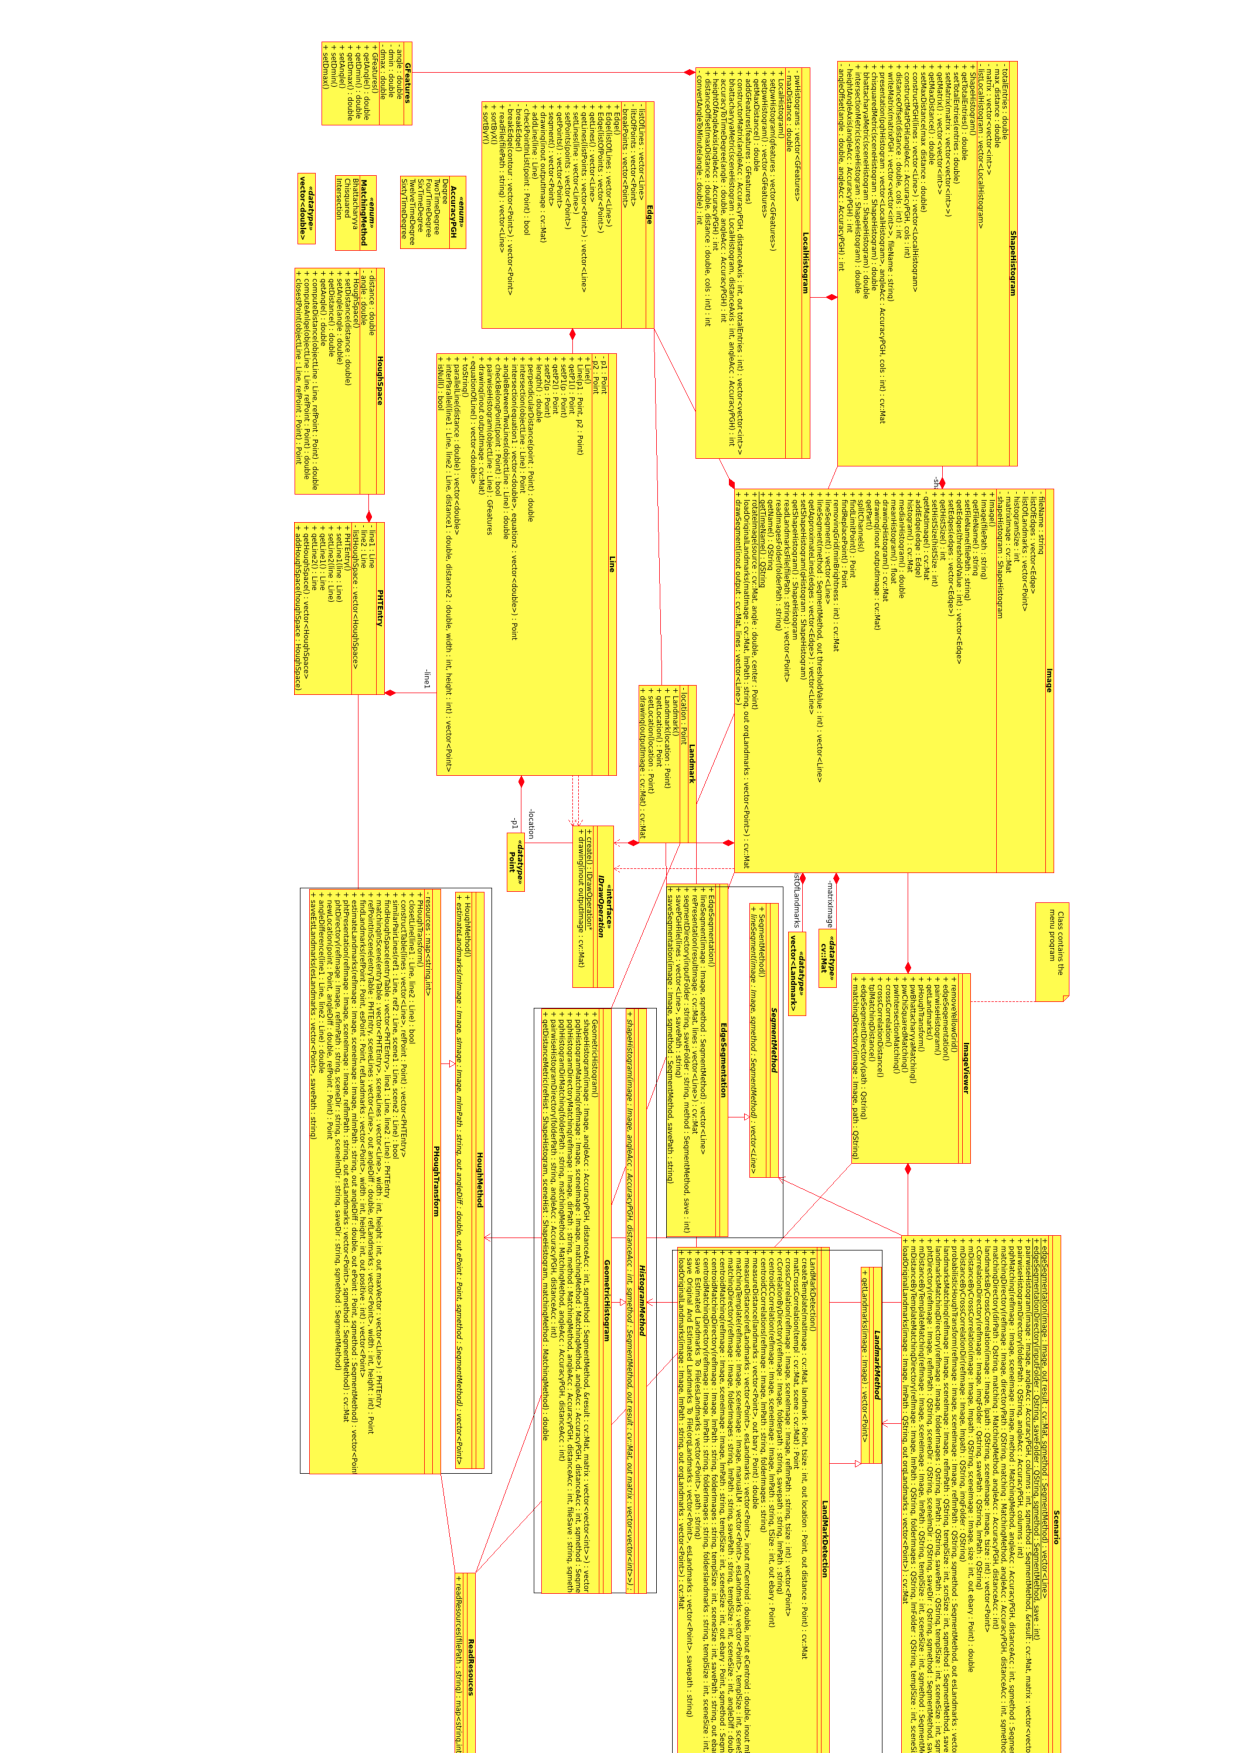
\includegraphics[width=1.1\linewidth]{images/cdiagram.pdf}
    }
    \caption{The class diagram diagram}
    \label{fig:cdiagram}
\end{figure}
The class diagram\footnote{See the full image in Appendix} in \ref{fig:cdiagram} show mainly classes of my task. The \textit{mainly} methods located in the \texttt{ImageViewer} class, where contains all functions of the software. To represent the information of image and preprocessing about clear the yellow grid, we use the classes such as \texttt{Line}, \texttt{Edge}, \texttt{Landmark}, \texttt{YellowGird}, \texttt{Image} class. For the edge segmentation, construct the pairwise geometric histogram, probabilistic hough transform and landmarks detection, we have \texttt{GFeatures}, \texttt{LocalHistogram}, \texttt{ShapeHistogram}, \texttt{EdgeSegmentation}, \texttt{PHTransform} \texttt{LandmarkDection} class. The main functions were inherated from the abstract classes \texttt{HistogramMethod}, \texttt{SegmentMethod}, \texttt{HoughMethod}, \texttt{LandmarkMethod} respective and used in \texttt{main} class (\texttt{ImageViewer}) via the \texttt{Sceneario} class. 
\section{Image preprocessing}
The \textit{Image processing} section describes the information about the classes which describe the geometric objects can be represent the image and the method to remove the yellow grid on the images.\\[0.2cm]
The \texttt{Line} class descibes the information of a straight line and its method, such as: get the length of line, compute the perpendicular distance from a point to line, find the intersection between two lines, compute the angle between two lines, find the parallel line with this line.\\[0.2cm]
The \texttt{Edge} class used to presented for a curve and the methods with edge. An edge can be presented by a list of lines or a list of points. The important methods in \texttt{Edge} class are \texttt{breakEdge()} and \texttt{segment()} method. It used to break the edge into approximate lines based on the list of point constructed edge.\\[0.2cm]
The \texttt{Image} class presented the information of an image such as file name, list of edge extracted from it. Besides, \texttt{Image} class also provides the methods to get the file name of image, compute the histogram of image, remove the yellow grid (if it exist) on image, get the PGH\footnote{Pairwise geometric histogram} of image, read its landmarks from a file, etc. \\[0.2cm]
\section{The abstract classes}
The abstract classes contains the abstract methods get the actions on image such as segmentation, PGH construction,.... The methods were implemented by the inherit classes, respective and provide the way access to action for other classes. The abstract classes include: \texttt{HistogramMethod} class, \texttt{SegmentMethod} class, \texttt{HoughMethod} class, \texttt{LandmarkMethod} class.
\section{Edge segmentation }
\texttt{Edge segmetation} includes the classes used for segment an image. Besides the classes construct the edge which described in previous section such as \texttt{Line, Edge,...}, we also provide the access method for another classes.\\[0.2cm]
The \texttt{EdgeSegmentation} class provides the methods such as obtain the lines from an image, presentation the result after segmentation or applying the segmentation on an images folder. The methods in \texttt{Edge segmentation} are:
\begin{itemize}
\item Extract the approximate lines of object in an image
\item Extract the approximate lines of object in each image in a folder
\end{itemize}
\section{Construct pairwise geometric histogram}
This section describes the classes used for PGH constructed process.\\[0.2cm]
\texttt{GFeatures} class contains the relative information of the objects in PGH such as angle, minimum distance and maximum distance. It provides the methods to get and set the relative information.\\[0.2cm]
\texttt{LocalHistogram} class constructed for containing the informations when computing the PGH of a line in object. The chosen lines as reference lines, the local histogram constructed based on recording the relative between reference line and other lines in object. Besides, it also have the methods help the user change the accuracy, such as the angle accuracy or distance accuracy.\\[0.2cm]
\texttt{ShapeHistogram} class constructs the PGH for an object. It was constructing based on combine all PGH of the lines in object. It also provides the methods to compute the measure distance between the pairwise geometric histograms by a matching method. The methods in this class includes:
\begin{itemize}
\item Construct the PGH for an image
\item Construct the matrix to save the PGH result
\item Compute the measure distance between two PGHs based on \textit{Bhattacharyya}, \textit{Chi-Squared} or \textit{Intersection} metric
\end{itemize}
\texttt{GeometricHistogram} class provides the access ways for another classes. By this class, the user can compute the pairwise geometric histogram of an image and calculate the distance between the pairwise geometric histograms.
\section{Estimate the global pose}
This section describes the classes use probabilistic hough transform to estimated a model image in a scene image. In particular is estimating the reference landmarks on the scene image.\\[0.2cm]
\texttt{HoughSpace} class contains the information about angle and distance from a line to a reference point. These information recorded to construct the accumulator when we apply the probabilistic hough transform.\\[0.2cm]
\texttt{PHTEntry} class present for each entry when constructing the reference table in training process. Each entry contains the pair of lines and its information about angle and distance to a reference point.\\[0.2cm]
\texttt{PHoughTransform} class describe the main process when we apply the probabilistic hough transform to estimate the landmarks. It includes the methods to construct the reference table, find the reference point in scene image and estimate the landmarks. Besides, it also provides the methods to estimated the landmarks of an image on directory of images.
\section{Refine the landmarks}
\texttt{LandmarkDetection} class provides the methods to refine the landmarks. It use cross-correlation technique to refine the estimated landmarks. Besides, we also can compute the centroid point of object.